\chapter[Introduction]{Introduction}
\label{ch:introduction}
\setcounter{footnote}{0}
The Greek philosopher Heraclitus once said that one constant since the beginning of time is change \parencite{Seibt2022}. However, the fear of change is also a constant. His central claim is summed up in the phrase Panta Rhei ("life is flux"), recognising life's essential, underlying essence as change. Nothing in life is permanent, nor can it be, because the very nature of existence is change. Since times \gls{immemorial}, humans have liked routine, making us feel in control of our lives. When the feeling of loosing control becomes irrational, the ability to control it can become a phobia \parencite{PsychTimes}. Someone with a phobia for change feels like they have no control over their lives due to constant change. These people tend to live in the past and are unwilling to progress, often leading to depression, seriously impacting their professional and personal lives. If a society or country rejects change, there could be no growth and progress \parencite{Mark2010}. The inability to change, progress, or grow can result in stagnation.

The Dutch \gls{ps} deals with many changes in its environment \parencite[p.~1]{Nijssen2018}. Changes follow one another at lightning speed. These are changes such as new technologies, social developments and political priorities. In the past, these were internal changes such as improving the financial and human resource processes, implementing a new way to organise and control, and the professionalisation of management processes \parencite[p.~13]{Eck2009}. In recent years, the external environment placed new and increasingly compelling demands on the functioning of public organisations. The \gls{ps} finds it challenging to adapt to the expected speed of change \parencites{Linders2013}[p.~2]{Wiebes2014}[pp.~5--6]{Auditdienst2019a}[p.~8]{Meijer2019}[pp.~1--2]{Tangi2020}. E.g. ''The processes, while solid, cannot withstand the current pace of change; the dependence on emergency solutions and manual work is increasing'' \parencite[p.~2]{Wiebes2014}. Trying to follow the expected speed of change often gets stuck on embedded norms, bureaucracy, processes, and structures \parencite[p.~1]{Tangi2020}. 

''There is a need to invest for an even a better government that can respond adequately and flexibly to unforeseen circumstances.'' was plead to Schippers\footnote{\url{https://en.wikipedia.org/wiki/Edith_Schippers}}\footnote{Schippers was at that time the appointed '\textit{informateur}' (Dutch). An '\textit{informateur}' is responsible to explore possible governing alliances after elections.} \parencite{Secretarissen-generaal2018}. A responsive and adaptive government is needed to deal with this \parencite[pp.~79--81]{Steen2018}. We need to create public organisations that can cope with or even seize opportunities in a dynamic difficult, unpredictable environment \parencite[pp.~1--2]{Nijssen2018}. In his essay, \textcite[p.~79]{Steen2018} tossed the concept \gls{antifragile} from \textcite{Taleb2012} as a possible direction to create an adaptive government.

\section{Introduction to antifragile}
\label{sec:introantifragility}
There are different manifestations to deal with uncertainty and disruptive changes \parencite[pp.~79--81]{Steen2018}. \Textcite{Steen2018} uses \textcite{Taleb2012} to discuss several manifestations for dealing with disruptive change. The five manifestations of \textcite{Taleb2012} provide a framework for the conversation about adaptive organisations \parencite[pp.~79--81]{Steen2018}. We have \gls{fragility}, \gls{robustness}, \gls{resiliency}, \gls{agility}, and \gls{antifragility}. Organisations that find it difficult or impossible to deal with changes are fragile. That does not mean that these organisations are not successful. They are often very sturdy, solid and successful. However, a fragile organisation will run into problems if the environment requires something from those organisations beyond the limits of the organisations capabilities. A \gls{robust} organisation absorbs and resists stress, while \gls{resilient} organisations move along with stress but bounce back to the status quo. \Gls{agile} organisations avoid stress just in time but do not gain, and with \gls{antifragility} an organisation gets better from stress. Agile is not acknowledged by \textcite{Taleb2012} and is in this context only used by \textcite{Steen2018}. \Gls{resiliency} is mentioned but \textcite{Taleb2012} only uses \gls{fragile}, \gls{robust}, and \gls{antifragile} for his \gls{triad} (\cref{fig:antifragilesimple}).
\begin{figure}[H]
	\centering
	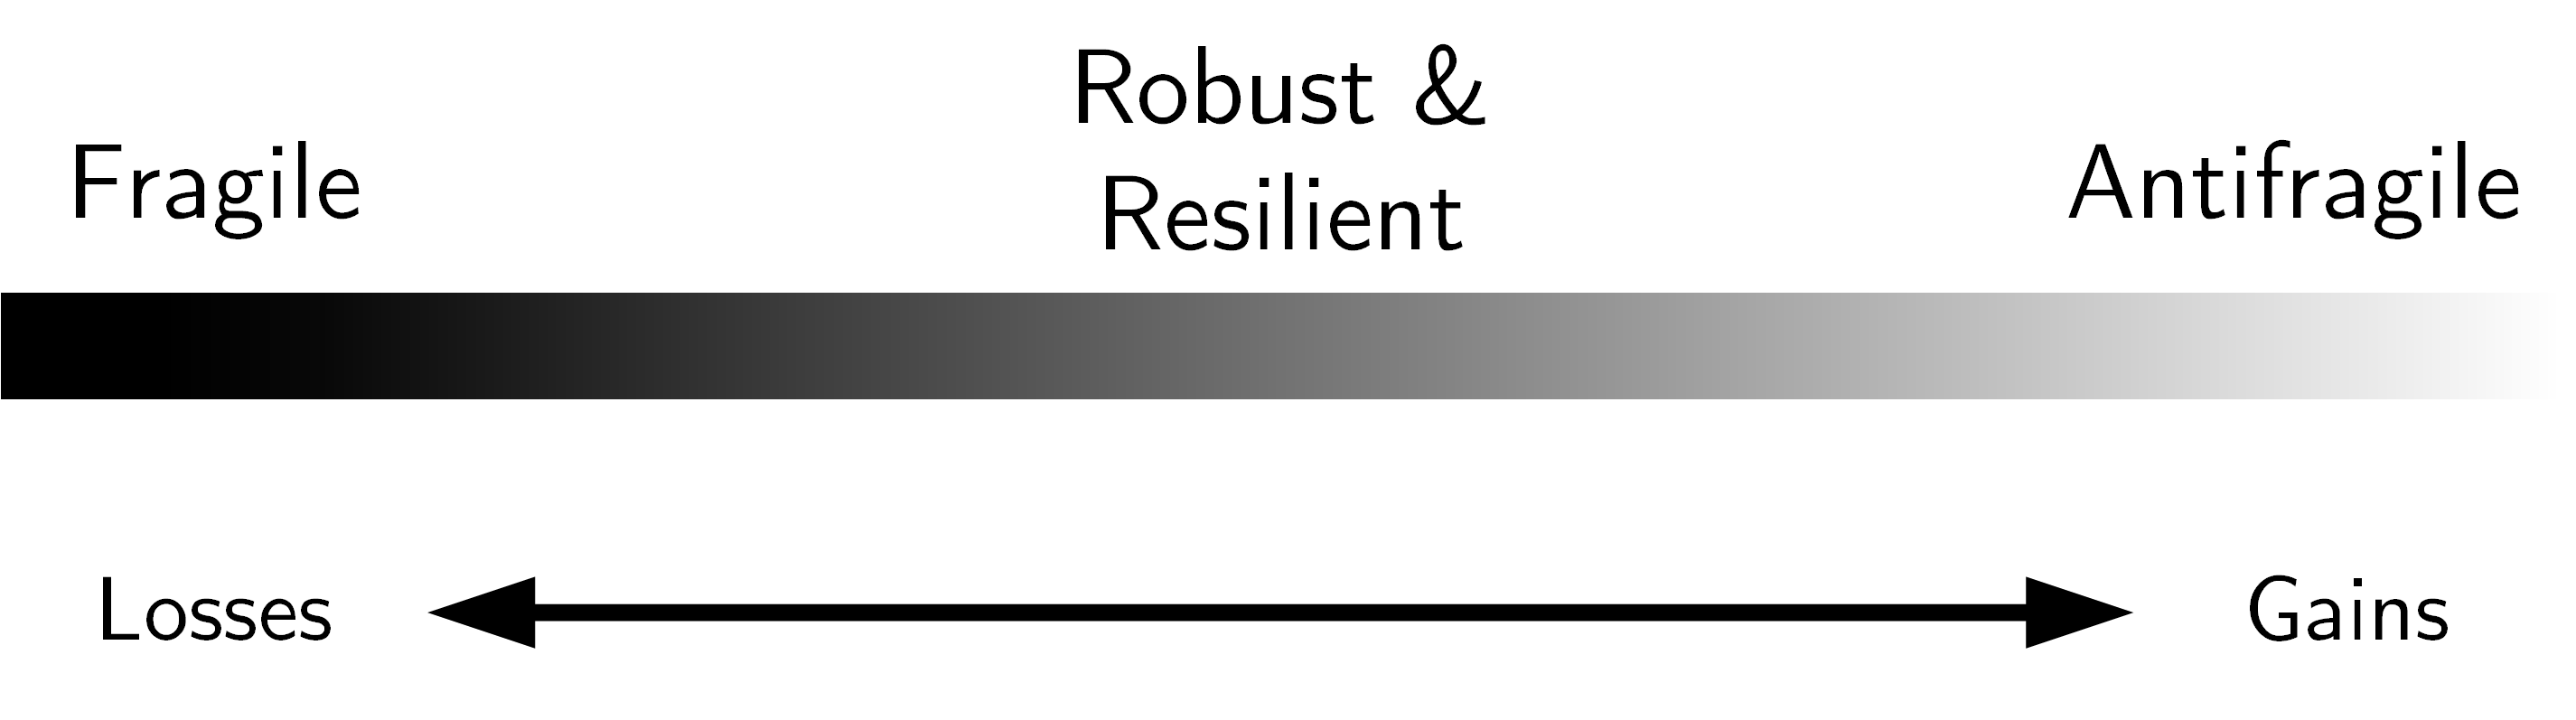
\includegraphics[width=0.6\linewidth]{images/antifragilesimple}
	\caption[The antifragile triad]{The antifragile triad}
	\label{fig:antifragilesimple}
\end{figure}
\textcite{Taleb2012} coined \gls{antifragile} as an answer to what he calls a \gls{blackswan}. \Glspl{blackswan} are large-scale unpredictable, and rare events of massive consequences \parencite[p.~6]{Taleb2012}. For extremely rare events the standard tools of probability and prediction, such as the normal distribution, do not apply since they depend on a large population and past sample sizes that are never available for rare events. \Gls{antifragile} means that a system gains more than it loses. 

\section{Introduction to Enterprise Architecture}
\label{sec:introea}
Due to the political and social environmental factors, the public sector deals continuously with changes and adjustments to objectives and missions \parencite{Nijssen2018}. This speed of change confronts policy-makers with high demands on their steering skills. The public sector started an improvement program for information provisioning \parencite{Digitaleoverheid2021} to deal with the increasingly compelling demands on the functioning of public organisations \parencite[p.~13]{Eck2009}. This program is a collaborative effort between governmental organisations, science, and suppliers \parencite[p.~128]{Digitaleoverheid2021}.

The improvement program positions, on multiple occasions, Enterprise Architecture as supportive of the proposed improvements, specifically the \acrfull{nora} and the \acrfull{ear}. \gls{ea}. E.g. ''Organisations can learn from previous experiences with the cross-organisational collaboration of the \acrlong{uwv}, and the Tax and Customs administration. The pillars and building blocks for chain management are part of the \acrshort{nora}.'' \parencite[p.~40]{Digitaleoverheid2021}. The governments defined \gls{ea} as ''Architecture that describes the current and future organisational management and the transformation path between them. \gls{ea} is a tool to manage the coherence between the various developments in the organisation.'' \parencite{NoraEA}. \acrshort{nora} and \acrshort{ear} are so called reference architectures.

A reference architecture describes general structures \parencite[p.~8]{Greefhorst2008}. It is not specific to one organisation. Many organisations can use a reference architecture because it is abstract. Abstract architectures are the basis for more specific architectures \parencite[p.~11]{Greefhorst2008}. They are an essential tool for reuse at an architectural level. Therefore, organisations should draw as much as possible from these architectures.

We deduct that there are multiple levels of architecture. Some kind of architecture hierarchy. Traditionally, reference architectures and \gls{ea} in the \gls{ps} correspond to the \acrshort{nora} terms of content \parencite{NORAfamilie}. These are reference architectures like \acrshort{ear} but also \acrfull{gemma}. The \acrshort{nora} itself is a daughter of the \acrfull{eira} (\cref{fig:architectureviewonion}).
\begin{figure}[H]
	\centering
	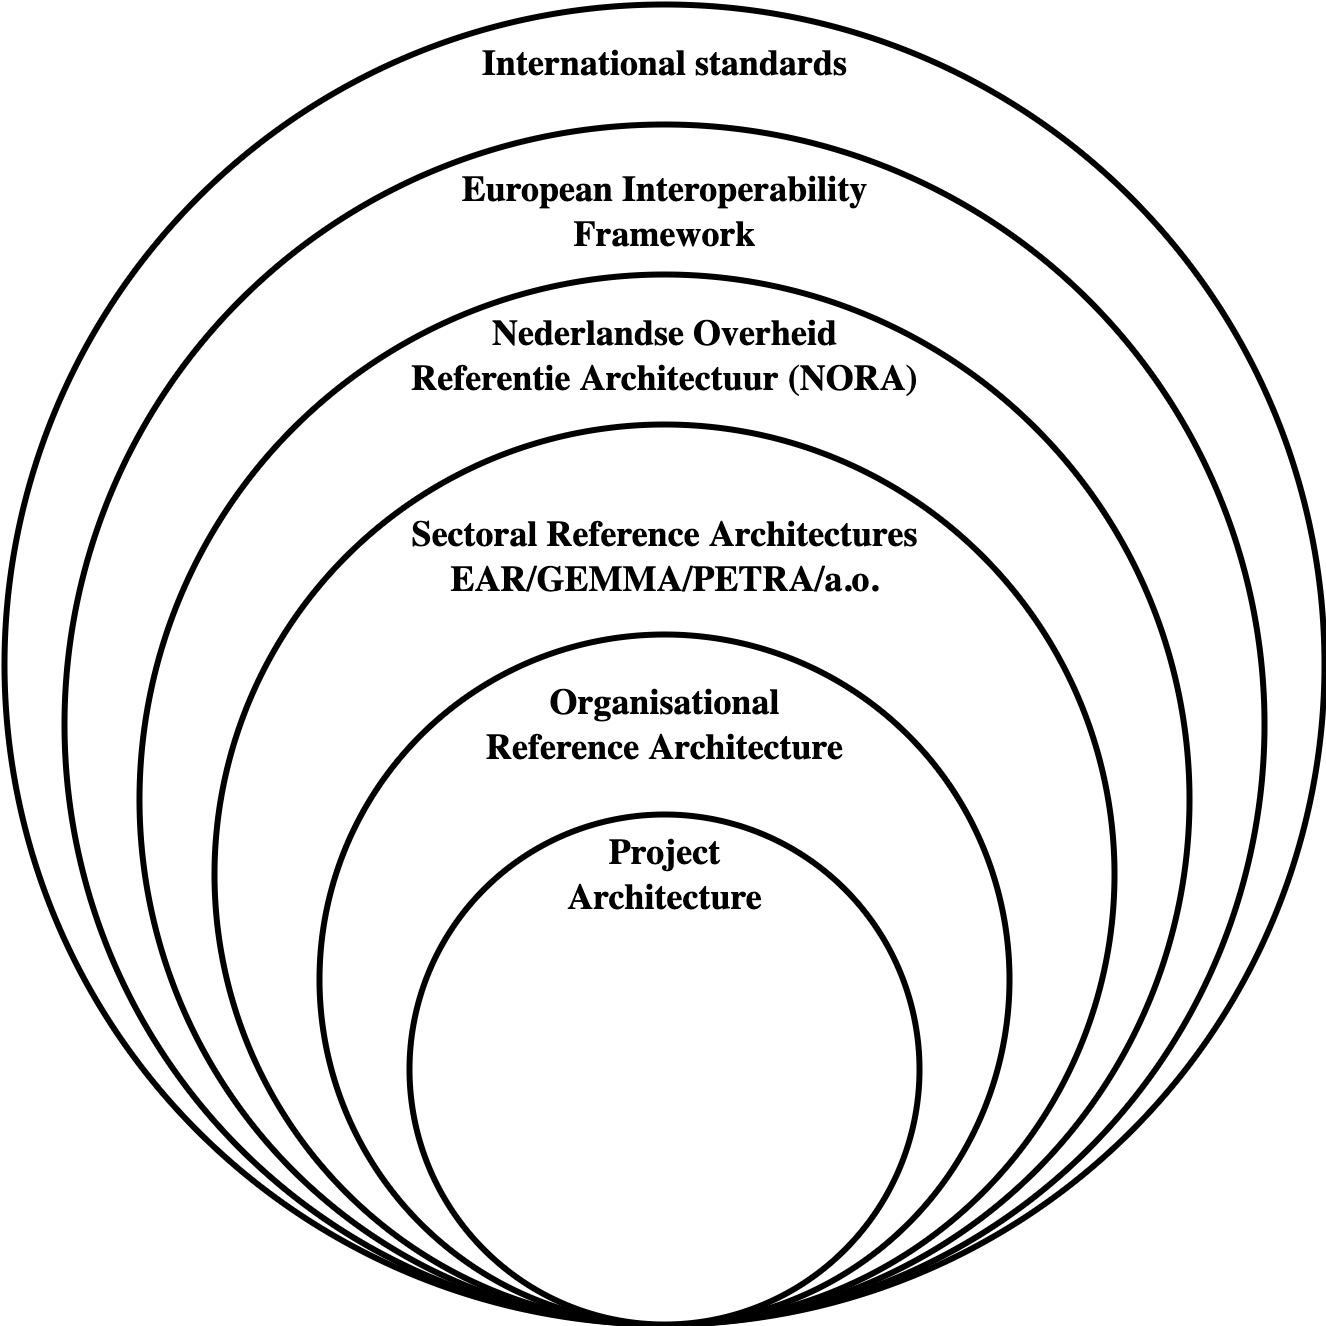
\includegraphics[width=0.5\linewidth]{images/architectureviewonion}
	\caption[Architecture subsidiaries, based on \textcite{Greefhorst2008}]{Architecture subsidiaries, based on \textcite{Greefhorst2008}}
	\label{fig:architectureviewonion}
\end{figure}
Changing higher-level reference architectures can support the 'I-strategy' improvement program. The changes ripple throughout the hierarchy. All the architectures correspond to the terms of the content of the higher architectures \parencite{NORAfamilie}. The central government uses \acrshort{ear} as a reference architecture. \acrshort{ear} is a subsidiary of \acrshort{nora}. The central government reactivates the 'Architecture Board Rijk' and the associated \acrshort{ear} for the improvement program \parencite[p.~42]{Digitaleoverheid2021}. The central government seeks collaboration with \acrshort{nora} for matching \acrshort{ear} with \acrshort{nora}.

\section{Research relevance}
\label{sec:researchrelevance}
The Dutch \gls{ps} wants to change toward being more adaptive and responsive (\cref{ch:introduction}). To be more adaptive and responsive, \textcite{Steen2018} proposed to use \gls{antifragile} from \textcite{Taleb2012} (\cref{sec:introantifragility}). \gls{ea} is defined as a tool by the Dutch \gls{ps} to support with the implementation of changes (\cref{sec:introea}). However, how can the Dutch \gls{ps} achieve \gls{antifragility} with support of \gls{ea}? What are \gls{antifragile} success factors relevant to the Dutch \gls{ps}, and what are \gls{ea} success factors in achieving it? The answer to these questions can make an impact on the Dutch \gls{ps}. These answers will support the Dutch \gls{ps} change itself to become more adaptive and responsive to better deal with unforeseen circumstances.

However, we could not find information on the combination of \gls{antifragile} and \gls{ea}. Let alone when we added the Dutch \gls{ps} or just the \gls{ps} context. Most research deals with \gls{antifragility} in application and information architectures. A small number of sources have investigated \gls{antifragility} in combination with organisations and systems. We have to discover these answers through research. We will research what the success factors are that positively influence becoming \gls{antifragile} with \gls{ea} in the Dutch \gls{ps}.

\section{Research model}
\label{sec:conceptualmodel}
There is little known about \gls{antifragility} and \gls{ea} in combination with the Dutch \gls{ps}.  When we decompose the statement we made in \cref{sec:researchrelevance}, we have a context of the Dutch \gls{ps} with two variables and a \gls{moderatorvariable}. We have the \gls{ea} as an \gls{independentvariable}, \gls{antifragile} as an \gls{dependentvariable}, and the success factors as an \gls{moderatorvariable} (\cref{fig:conceptualmodel}). Our hypothesis is that there are factors that have a positive influence on achieving \gls{antifragility} in the Dutch \gls{ps} with \gls{ea}.
\begin{figure}[H]
	\centering
	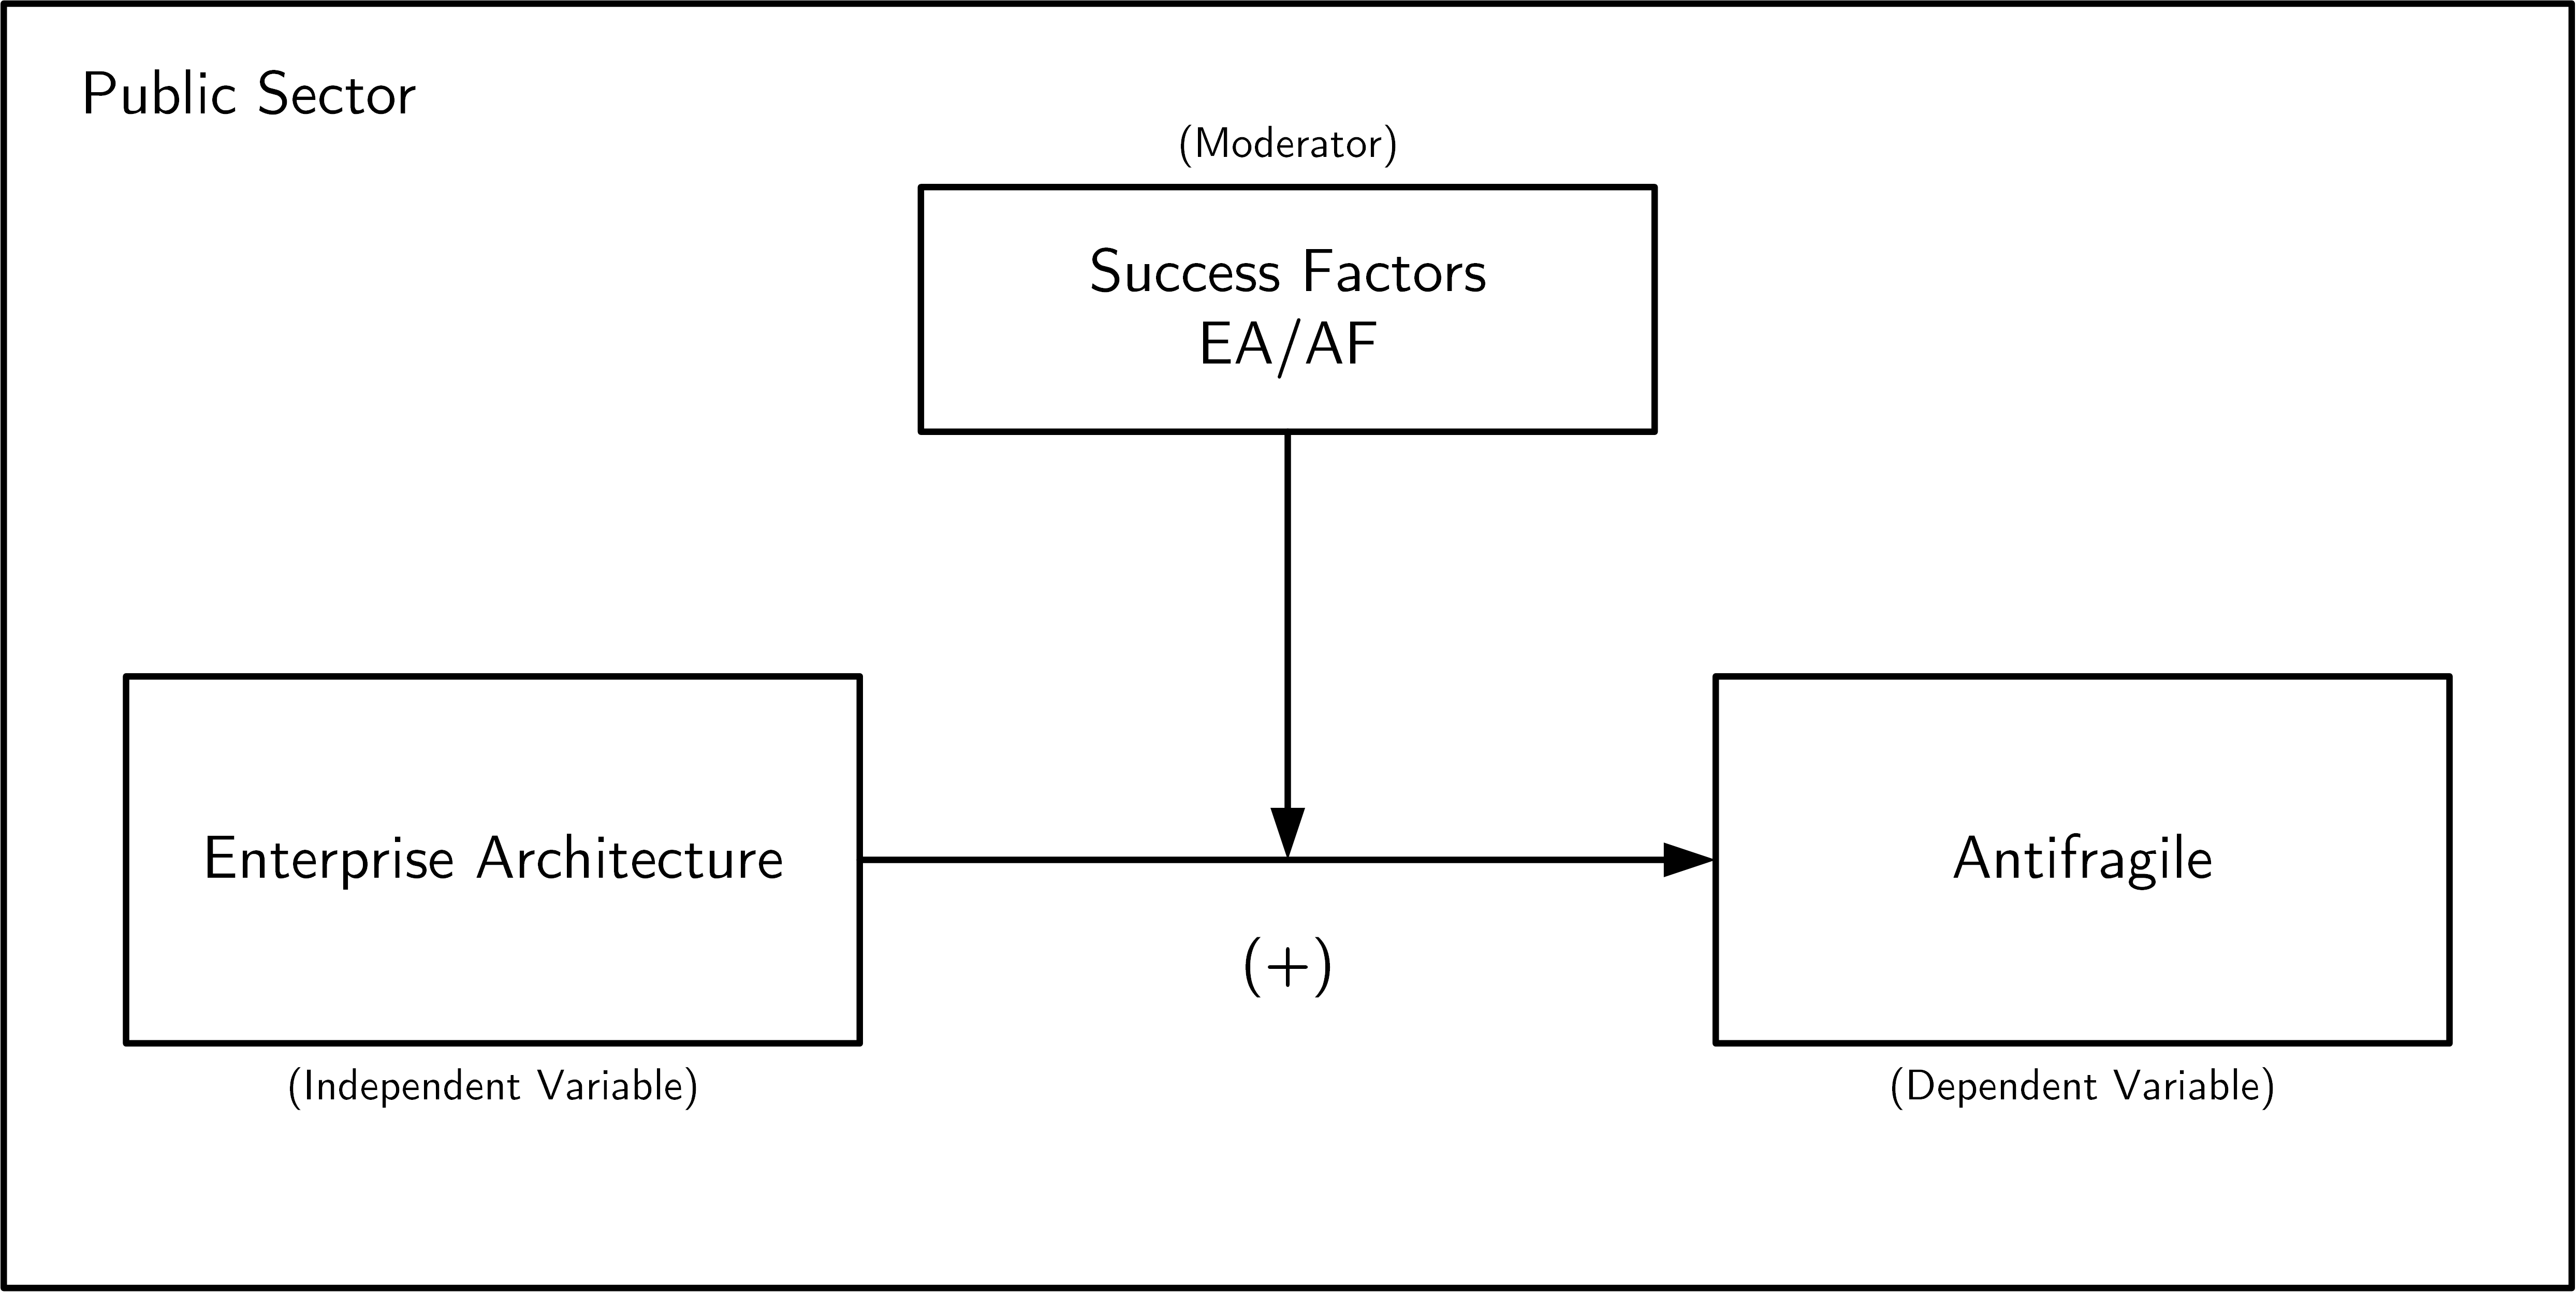
\includegraphics[width=0.7\linewidth]{images/conceptualmodel}
	\caption[Conceptual Research Model]{Conceptual Research Model}
	\label{fig:conceptualmodel}
\end{figure}

\section{Research question}
\label{sec:introresearchquestion}
Our hypothesis is that there are factors that have a positive influence on achieving \gls{antifragility} in the Dutch \gls{ps} with \gls{ea} (\cref{fig:conceptualmodel}). Following the conceptual research model, we have the following research question:

\vspace{\baselineskip}
\noindent \emph{'What are success factors of \gls{ea} and \gls{antifragile} that positively influence the contribution of \gls{ea} in achieving \gls{antifragility} in the Dutch \gls{ps}?'}
\vspace{\baselineskip}

\noindent The following sub-questions support answering the research question:
\begin{enumerate}
	\item{What is the Dutch \gls{ps}?}
	\item{What is \gls{antifragile}?}
	\item{What are success factors for \gls{antifragility}?}
	\item{What is \gls{ea}?}
	\item{What are success factors of \gls{ea}?}
	\item{Which success factors are relevant for the Dutch \gls{ps}?}
\end{enumerate}

\section{Thesis design}
\label{sec:structure}
The structure of this thesis follows a pattern of divergence before convergence (\cref{fig:design}). We introduce the research (\cref{ch:introduction}). We present the context, explain the design of the thesis, and the necessity of the research. Following, we introduce the main concepts of the research together with a problem statement and research questions. We give a background on the concepts of the research (\cref{ch:theoreticalbackground}). This part also contains the outcome of the literature research we performed based on the approach described in the methodology (\cref{ch:methodology}). The methodology explains the research design, the methods, the quality and the approach. All of these are part of the divergence of the research. We collected much data, but we still have to validate the data and narrow it down to formulate an answer to our research question. The second part of the thesis design will converge the findings.
\begin{figure}[H]
	\centering
	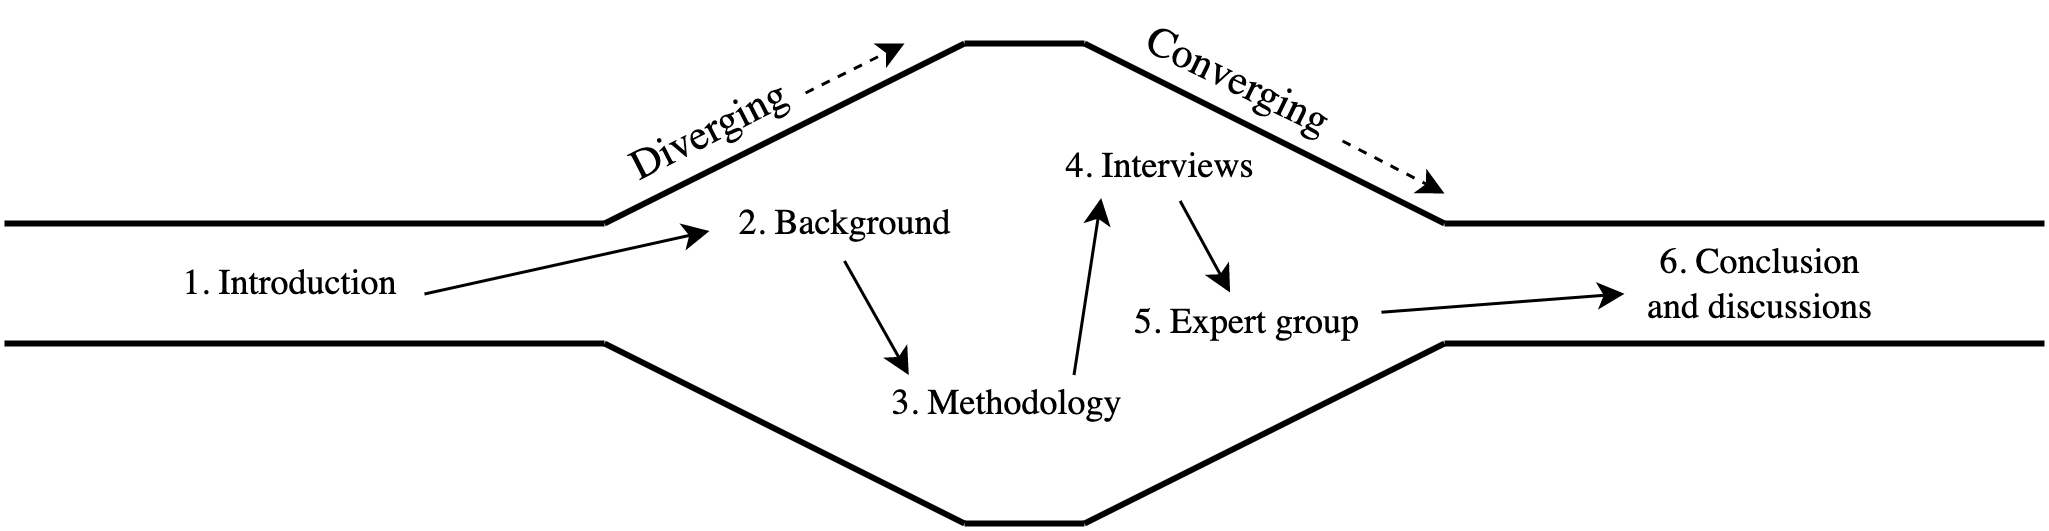
\includegraphics[width=0.9\linewidth]{images/structure}
	\caption[Design of the thesis]{Structure of the thesis}
	\label{fig:design}
\end{figure}
We validate findings with interviews (\cref{ch:interviews}) and an expert group (\cref{ch:expertgroup}). Converging ends with  conclusion and discussions (\cref{ch:conclusionanddiscussions}). This chapter contains also the limitations of the research and a retrospective. We have a glossary of terms available at the tail of the thesis to support the reader with used definitions.
